\documentclass[a4paper,german]{scrreprt}

% Uncomment to optimize for double-sided printing.
% \KOMAoptions{twoside}

% Set binding correction manually, if known.
% \KOMAoptions{BCOR=2cm}

% Localization options
\usepackage[german]{babel}
\usepackage[T1]{fontenc}
\usepackage[utf8]{inputenc}

% Enhanced verbatim sections. We're mainly interested in
% \verbatiminput though.
\usepackage{verbatim}

% PDF-compatible landscape mode.
% Makes PDF viewers show the page rotated by 90°.
\usepackage{pdflscape}

% Advanced tables
\usepackage{tabu}
\usepackage{longtable}
\usepackage{dcolumn}
\newcolumntype{d}[1]{D{.}{\cdot}{#1} }

% Fancy tablerules
\usepackage{booktabs}

% Graphics
\usepackage{graphicx}

% Current time
\usepackage[useregional=numeric]{datetime2}

% Float barriers.
% Automatically add a FloatBarrier to each \section
\usepackage[section]{placeins}

% Custom header and footer
\usepackage{fancyhdr}

\usepackage{geometry}
\usepackage{layout}

% Math tools
\usepackage{mathtools}
% Math symbols
\usepackage{amsmath,amsfonts,amssymb}
\usepackage{amsthm}

% SI units
\usepackage{siunitx}
\DeclareSIUnit\Molar{\textsc{m}}

% Chemistry
\usepackage{mhchem}

% Subfigures & captions
\usepackage{subcaption}

\DeclarePairedDelimiter\abs{\lvert}{\rvert}

\pagestyle{plain}
% \fancyhf{}
% \lhead{}
% \lfoot{}
% \rfoot{}
% 
% Source code & highlighting
\usepackage{listings}

% Convenience commands
\newcommand{\mailsubject}{2027 - Praktikum Biochemie 1}
\newcommand{\maillink}[1]{\href{mailto:#1?subject=\mailsubject}
                               {#1}}

% Should use this command wherever the print date is mentioned.
\newcommand{\printdate}{\today}

\subject{2027 - Praktikum Biochemie 1}
\title{9 - Reinigung von Proteinen mittels Chromatographie}

\author{Michael Senn \maillink{michael.senn@students.unibe.ch} - 16-126-880}

\date{\printdate}

% Needs to be the last command in the preamble, for one reason or
% another. 
\usepackage{hyperref}


\begin{document}
\maketitle

\chapter{Einleitung}

\section{Zielsetzung}

Ziel des Experimentes war es, ein Kartoffel-Protein-Gemisch mittels
Chromatographie aufzutrennen und die resultierenden Phasen auf
Katalase-Aktivität zu untersuchen.

\section{Chromatographie von Proteinen}

Zwecks Auftrennung eines Proteingemisches in die einzelnen Proteine, oder
Extrahierung eines bestimmten Proteins, existieren verschiedene Methoden. Eine
solche Gruppe von Methoden ist die Chromatographie.

In der Chromatographie werden Wechselwirkungen zwischen den zu trennenden
Proteinen, und anderen Chemikalien, ausgenutzt. Dies können beispielsweise
nicht-kovalente spezifische Bindungen sein, ionische Wechselwirkungen,
unterschiedliche Löslichkeiten in verschiedenen Lösungsmitteln usw. Diese
Unterschiede erlauben, das Proteingemisch kontrolliert in dessen Bestandteile
zu zerlegen.

Hierzu wird ein hohler schlauförmiger Behälter - Säule genannt - mit zwei
Phasen gefüllt. Die stationäre Phase - beispielsweise als Beschichtung im
Säuleninnere oder festes Füllmaterial der Säule - ist entsprechend ihrem Namen
unbeweglich im Säuleninnere. Die mobile Phase - beispielsweise als Flüssigkeit
- durchläuft die Säule und trägt dabei das aufzutrennende Gemisch mit.

Je nach Wechselwirkungen der einzelnen Proteine mit der mobilen und/oder
stationären Phase, durchlaufen diese die Säule mit einer unterschiedlichen
Geschwindigkeit und werden so, zeitlich versetzt, die Säule verlassen.

\subsection{Ionenaustauschchromatographie}

In der Ionenaustauschchromatographie wird als stationäre Phase ein
Ionentauscher verwendet. Dieser bindet, im Falle eines Anionentauschers negativ
geladene, im Falle eines Kationentauschers positiv geladene, Proteine.

Nach Durchlauf der Probe sind damit alle entsprechend geladenen Proteine in der
stationären Phase gebunden. Anschliessend wird die Säule mit dem Eluenten
gespült. Dessen Ionen stehen in Konkurrenz mit den an die stationäre Phase
gebundenen Ionen und führen so - je nach Konzentration des Eluenten - dazu,
dass sich gewisse der gebundenen Proteine lösen, und aus der Säule ausgewaschen
werden.

Da sich zuerst jene Proteine lösen, die am schwächsten an die
Ionenaustaschmatrix binden, kann damit durch die kontrollierte Erhöhung der
Konzentration des Eluenten - Gradient genannt - das gebundene Proteingemisch in
einzelne Phasen, geordnet nach Ladung, getrennt werden.

\subsection{Einfluss des pH auf die Protein-Ladung}

Die Ladung des Proteins wird von gewissen Seitenketten beeinfluss, welche
unterschiedlich gut protonierbar sind. Damit beinflusst der Arbeits-pH direkt
die Ladung des Proteins. Bei einem gewissen pH Wert - isoelektrischer Punkt pI
genannt - ist das Protein ungeladen. Bei höherem Arbeits-pH ist das Protein
negativ geladen und bindet somit an eine Anionenaustauschmatrix, bei tiererem
Arbeits-pH ist es positiv geladen, und bindet an eine Kationenaustauschmatrix.

\section{Nachweis der Katalase-Aktivität}

Zwecks Nachweis von Katalase in den Fraktionen dient eine Reaktion von
\ce{H2O2} mit ABTS welche, durch eine Peroxidase katalysiert, zur Bildung eines
grünen, in Lösung einfach zu erkennenden, Stoffes führt.

In Fraktionen in denen Katalase vorhanden ist, ist zu erwarten dass \ce{H2O2}
abgebaut wird, und sich bei Zugabe von ABTS keine Grünfärbung einstellt. Stellt
sich eine Grünfárbung ein, deutet dies darauf hin, dass ungenügend Katalase
vorhanden war, um alles \ce{H2O2} abzubauen.

Die beiden miteinander konkurrenzierenden Reaktionsmechanismen sind somit:
\begin{itemize}
	\item Der Abbau von \ce{H2O2} durch Katalase: \ce{2 H2O2 ->T[Katalase] 2 H2O + O2}
	\item Die Bildung der oxidierten Form von ABTS katalysiert durch eine
		Peroxidase: \ce{H2O2 + ABTS_{red, (farblos)} ->[Peroxidase]
		ABTS(O)_{ox, (grün)} + H2O}
\end{itemize}

Mittels serieller Verdünnung, und Vergleich mit einer Katalse-Lösung mit
bestimmter Konzentration, kann zusätzlich von jeder Fraktion die
Katalse-Konzentration abgeschätzt werden.


\section{Apparaturschema}

\begin{figure}[h]
	\centering
	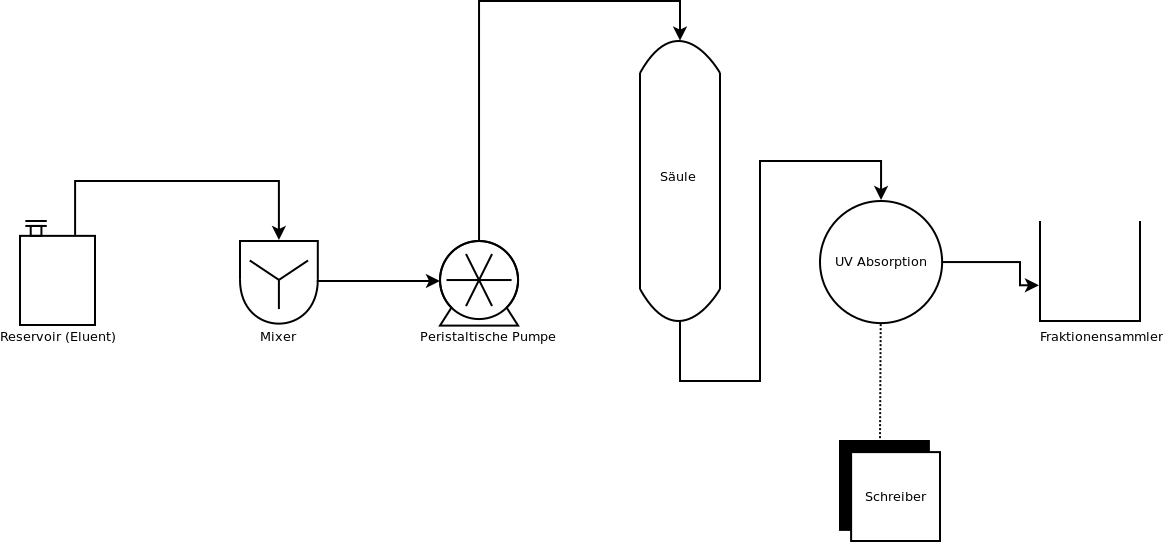
\includegraphics[width=0.9\textwidth]{img/apparatur.png}
	\caption{Apparatur für Ionenaustauschchromatographie}
	\label{fig:apparatur}
\end{figure}

Abbildung \ref{fig:apparatur} ist eine systematische Darstellung der
verwendeten Versuchsapparatur, mit welcher die Ionenaustauschchromatographie
durchgeführt wurde.

\chapter{Material \& Chemikalien}

\section{Material}

\begin{itemize}
	\item 1 Styroporbox mit Eis
	\item Schnitzer und Kartoffeln
	\item 1 Mixer
	\item 1 Sorvallzentrifuge und SS34 Rotor
	\item 2 Sorvallzentrifugen-Röhrchen
	\item 1 \SI{500}{ml}, 2 \SI{100}{ml} Becherglas
	\item 2 \SI{500}{ml} Duran Flaschen
	\item 1 Säule
	\item 1 Peristaltische Pumpe
	\item 1 Fraktionensammler
	\item 1 UV-Detektor
	\item 1 Schreiber
	\item 1 Magnetrührer
	\item 1 kleiner linearer Gradientenmischer
	\item 1 Mikrotiterplatte
	\item 1 12-Kanalpipeppte mit Spitzen
\end{itemize}

\section{Chemikalien \& Lösungen}

\begin{itemize}
	\item  \SI{1}{\Molar} \ce{TRIS-HCl}, pH 7.75
	\item \ce{NaCl}
	\item Puffer A: \SI{20}{\milli\Molar} \ce{TRIS-HCl}, pH 7.75
	\item Puffer B, Eluent: Puffer A + \SI{1}{\Molar} \ce{NaCl}
	\item ABTS-Stocklösung in \ce{H2O}, \SI{50}{\milli\gram \per \milli\litre}
	\item Horse radish peroxidase, HR-POX: Aktivität ca \SI{700}{U \per \milli\gram}
	\item Bovine liver catalase: Aktivität \SI{2088}{U \per \milli\gram}
	\item \ce{H2O2} \SI{30}{\percent} in \ce{H2O}
	\item Magermilchpulver
\end{itemize}

\chapter{Durchführung}

\chapter{Resultate}

\chapter{Diskussion}

\bibliographystyle{plain}
\bibliography{references}

\end{document}
